% /* cSpell:enable */
% /* cSpell:locale de,en */
\chapter{Umfrage}
\label{cha:umfrage}

Durch die Umfrage sollte die Bedeutung des Wortes Wirksamkeit in der Bevölkerung sowie die Einordnung der COVID-19-Impfung geklärt werden. Der Fragebogen besteht aus insgesamt 27 Fragen, davon sechs Fragen zur Erhebung über die Stichprobe. Die Ergebnisse wurden auf GitHub\footnote{\hyperlink{https://github.com/andreaseckmayr/BachelorThesis/blob/main/survey/Fragebogen\%20-\%20Wirksamkeit\%20d.\%20Covid-19\%20Impfung\%20(Responses)\%20-\%20Form\%20responses\%201.csv}{https://github.com/andreaseckmayr/BachelorThesis}} veröffentlicht.

\section{Methodik}

Die Umfrage wurde mit Google Forms erstellt. Die Stichprobengröße betrug 425 Personen und ergab sich durch Befragung des erweiterten Bekanntenkreises in den Gebieten Eferding und Purkersdorf. Die Umfrage wurde per Twitter, Facebook und WhatsApp verbreitet und online vom 14. April bis 1. Mai durchgeführt.
Das Alter der TeilnehmerInnen lag zwischen 14 und 83, dabei betrug der Mittelwert 47 Jahre und der Median 48 Jahre, der Modus 52 Jahre. 31\% der TeilnehmerInnen waren Männer, 69\% Frauen.
Im Vergleich dazu liegt das Durchschnittsalter der Bevölkerung in Österreich bei 43,1 Jahren, der Frauenanteil liegt bei 50,7\%.

\begin{figure}[hp]
    \centering
    \begin{tikzpicture}
        \pie[
            %color = {
            %    yellow!90!black,
            %    green!60!black,
            %    blue!60,
            %    red!70, 
            %    gray!70,
            %    teal!20},
            %hide number,
            text=legend,
            radius=2
        ]{
            31.1/männlich,
            68.7/weiblich,
            0.2/divers
        }
    \end{tikzpicture}
    \caption{Geschlechtsverteilung}
\end{figure}

\newpage

Betrachtet man die Stichprobe nach abgeschlossener Bildung, so stellt sie sich wie folgt dar:
\begin{itemize}
    \item 52\% haben eine Hochschule oder Universität abgeschlossenen
    \item 25\% haben eine Matura als höchste Ausbildung
    \item 11\% haben eine berufsbildende mittlere Schule (BMS) abgeschlossenen
    \item 10\% haben eine Lehre abgeschlossenen
    \item 2\% haben einen Pflichtschulabschluss
    \item weniger als 1\% hat noch keinen Abschluss
\end{itemize}

\begin{figure}[hp]
    \centering
    \begin{tikzpicture}
        \pie[
            %color = {
            %    yellow!90!black,
            %    green!60!black,
            %    blue!60,
            %    red!70, 
            %    gray!70,
            %    teal!20},
            %hide number,
            text=legend,
            radius=2.5
        ]{
            51.5/Hochschule; Universität,
            25.4/AHS; BHS; Abendmatura,
            10.6/BMS (Fach- od. Handelsschule),
            10.1/Lehre,
            1.9/Pflichtschule,
            0.5/noch kein Abschluss
        }
    \end{tikzpicture}
\caption{Höchste abgeschlossene Ausbildung}
\end{figure}

Gefragt wurde auch nach dem aktuellem Beruf. Dabei gaben zwei Drittel der Befragten an, unselbstständig angestellt zu sein. Davon sind 20\% leitende Angestellte und 4\% ArbeiterInnen. Jeweils ca. 15\% sind selbstständig oder derzeit nicht erwerbstätig und 5\% befinden sich noch in Ausbildung. Insgesamt 14\% der Befragten sind im Gesundheitsbereich tätig.

\begin{figure}[hp]
    \centering
    \begin{tikzpicture}
        \pie[
            %color = {
            %    yellow!90!black,
            %    green!60!black,
            %    blue!60,
            %    red!70, 
            %    gray!70,
            %    teal!20},
            %hide number,
            text=legend,
            radius=2.5
        ]{
            49.4/Angestellt,
            13.9/Leitendende Anstellung,
            2.8/ArbeiterIn,
            14.8/derzeit nicht erwerbstätig,
            14.6/Selbstständig,
            4.5/in Ausbildung
        }
    \end{tikzpicture}
\caption{Erwerbstätigkeit}
\end{figure}

\section{Ergebnisse}

\subsection{Impfwilligkeit und Wirksamkeit}

Um die Impfwilligkeit einzuschätzen, wurden die Teilnehmer befragt, unter welchen Umständen sie sich impfen lassen würden. Dabei stimmte der Aussage, sich gegen Krankheiten mit hohem Infektionsrisiko, aber leichten Krankheitssymptomen impfen zu lassen, ein Viertel gar nicht oder eher nicht zu, ein Fünftel war unentschlossen und 54\% stimmten eher bzw. völlig zu. Der konträren Aussage, sich gegen Krankheiten mit niedrigem Infektionsrisiko, allerdings schweren Krankheitssymptomen würde sich nur ein Zehntel nicht oder eher nicht impfen lassen, 13\% sind noch unentschlossen und 77\% antworteten mit ja oder eher ja.

Kurzzeitige Nebenwirkungen würden die meisten Menschen in Kauf nehmen, wobei fast 90\% leichte und 61\% auch noch schwere Nebenwirkungen akzeptieren würden. Länger andauernde Nebenwirkungen würde nur noch ein Viertel der Teilnehmer in Kauf nehmen.

Während 70\% der Befragten noch auf Empfehlungen der eigenen Ärztin oder des eigenen Arztes achten, gaben nur 61\% an, auch auf die Empfehlungen des Gesundheitsamtes oder der Impfkommission zu hören. 21\% waren gar der Meinung, auf die Empfehlung der Impfkommission eher nicht oder überhaupt nicht zu achten.

\begin{table}[h!]
    \centering
    \begin{tabular} {p{7.5cm} r r r r r}
        & 1 & 2 & 3 & 4 & 5 \\
        \hline
        Ich würde mich gegen Krankheiten mit\ldots & & & & & \\
        - hohem Infektionsrisiko, jedoch leichten Symptomen impfen lassen & 14,8\% & 12,0\% & 19,3\% & 20,7\% & 33,2\% \\

        - niedrigen Infektionsrisiko, jedoch schweren Symptomen impfen lassen & 5,6\% & 4,7\% & 12,9\% & 18,6\% & 58,1\% \\

        \\

        In Kauf nehme ich\ldots & & & & & \\

        - kurzzeitige leichte Nebenwirkungen wie Müdigkeit oder Schwindel & 2,8\% & 4,2\% & 5,4\% & 13,2\% & 74,4\% \\

        - kurzzeitige schwere Nebenwirkungen wie hohes Fieber & 10,4\% & 10,6\% & 18,1\% & 32,0\% & 28,9\% \\

        - länger andauernde Nebenwirkungen wie Müdigkeit & 20,5\% & 22,6\% & 28,7\% & 18,6\% & 9,6\% \\

        \\

        Vor einer Impfung achte ich auf\ldots & & & & & \\

        - Empfehlungen meiner Ärztin bzw. meines Arztes & 2,6\% & 8,0\% & 19,3\% & 28,7\% & 41,1\% \\

        - Empfehlungen des Gesundheitsamtes oder der Impfkommission & 9,9\% & 11,3\% & 17,9\% & 31,1\% & 29,9\% \\
    \end{tabular}
    \caption{Impfwilligkeit - Übersicht (1=ich stimme gar nicht zu, 5=ich stimme völlig zu)}
    \label{tab:impfwilligkeit}
\end{table}

Um wirksam zu sein, muss eine Impfung für fast 90\% der Befragten zumindest die Symptome mildern. Etwas weniger Zustimmung gab es zur Aussage, eine Impfung müsse das Infektionsrisiko senken (84\%) sowie die Wiedergabe des Erregers verhindern (80\%).

\begin{table}[h!]
    \centering
    \begin{tabular} {p{7.5cm} r r r r r}
        & 1 & 2 & 3 & 4 & 5 \\
        \hline
        Für mich ist eine Impfung wirksam\ldots & & & & & \\

        - wenn sie mein Infektionsrisiko senkt & 1,9\% & 4,2\% & 9,9\% & 26,6\% & 57,4\% \\

        - wenn sie die Weitergabe des Krankheitserregers verhindert & 2,1\% & 4,0\% & 13,9\% & 25,4\% & 54,6\% \\

        - wenn sie im Falle einer Infektion meine Symptome mildert & 2,1\% & 2,8\% & 8,0\% & 23,8\% & 63,3\% \\
    \end{tabular}
    \caption{Wirksamkeit - Übersicht (1=ich stimme gar nicht zu, 5=ich stimme völlig zu)}
    \label{tab:wirksamkeit}
\end{table}

\subsection{Gründe für eine Nicht-Impfung}

Zunächst wurden ungeimpfte Teilnehmer gefragt, was der Grund für eine Nicht-Impfung sei. Dabei standen folgende Antwortmöglichkeiten zur Auswahl:
\begin{itemize}
    \item religiöse Gründe
    \item gesundheitsbedingte Gründe
    \item generell vorsichtige Einstellung gegenüber Impfungen
    \item Angst vor Nebenwirkungen
\end{itemize}
Zwei Drittel der Befragten (62,9\%) gab an, Impfungen gegenüber generell vorsichtig eingestellt zu sein.
Rund ein Fünftel (22,9\%) gab an, Angst vor Nebenwirkungen zu haben.
14,3\% der TeilnehmerInnen gab gesundheitsbedingte Gründe an, die Religion war für keine Person Grund, sich nicht impfen zu wollen.
Diese Ergebnisse spiegeln sich teilweise in einer früheren forsa-Befragung wieder, in der knapp 18\% ebenfalls Angst vor Nebenwirkungen und 8\% gesundheitliche Gründe oder Schwangerschaft bzw. Stillzeit (5\%) angaben. Damals gaben allerdings lediglich 2\% Skepsis bzw. Ablehnung von Impfungen an, jedoch 34\% hielten Impfstoffe für nicht ausreichend erprobt. \cite{forsa-befragung}

\subsection{Gründe für eine Impfung}

Der Großteil der TeilnehmerInnen war zum Zeitpunkt der Umfrage bereits gegen COVID-19 geimpft. 81\% hatten die dritte Impfdosis -- den sogennanten Booster -- erhalten, 7\% wurden zwei mal geimpft. 9\% der Befragten waren noch ungeimpft.

Von den geimpften Personen haben sich vier Fünftel zum ehestmöglichen Zeitpunkt impfen lassen, 14\% haben einige Wochen verstreichen lassen und auf Reaktionen aus dem Freundes- und Bekanntenkreis gewartet. Zirka 3\% gab die Einführung von 3G am Arbeitsplatz, 1,6\% die Einführung von 2G in Gastronomie und Einzelhandel als Zeitpunkt an der Impfung an.

Nach den Gründen gefragt, war für beinahe 90\% der Selbstschutz ausschlaggebend, 76\% wollten besonders vulnerable Personengruppen schützen.  Leichter Reisen zu können war für ein Fünftel ein Impfgrund. 6\% gaben hier an, dass die 3G-Pflicht am Arbeitsplatz die Entscheidung beeinflusst hat, 5\% die 2G-Pflicht in Gastronomie und Einzelhandel.

\begin{table}[h!]
    \centering
    \begin{tabular} {p{12,5cm} r}
        Wann haben Sie sich impfen lassen? & \\
        \hline

        - Zum ehestmöglichen Zeitpunkt & 80,2\% \\

        - Nach ein paar Wochen, als bereits einige Freunde und Bekannte geimpft waren & 14,3\% \\

        - Mit der Einführung von 3G am Arbeitsplatz & 2,9\% \\

        - Mit der Einführung von 2G in der Gastronomie und im Handel & 1,6\% \\

        - Nach ein paar Wochen, aber aus dem Bekannten- und Familienkreis war ich der/die Erste & 1,0\% \\ \\

        Aus welchem Grund haben Sie sich impfen lassen? & \\
        \hline

        - Zu meinem eigenem Schutz & 88,8\% \\

        - Um besonders gefährdete Menschen zu schützen & 75,5\% \\

        - Um einfacher Reisen zu können & 17,5\% \\

        - Aufgrund der 3G-Pflicht am Arbeitsplatz & 5,5\% \\

        - Aufgrund der 2G/3G-Pflicht in Gastronomie und Handel & 5,2\% \\
    \end{tabular}
    \caption{Zeitpunkt der und Gründe für die COVID-19-Impfung - Übersicht}
    \label{tab:gruende}
\end{table}

\subsection{Vertrauen und Wirksamkeit bezüglich COVID-19-Impfung, Hygienemaßnahmen und Verordnungen}

Zuletzt wurden die TeilnehmerInnen gefragt, in welchen Bereichen Sie der COVID-19-Impfung vertrauen bzw. nicht vertrauen. Diese Bereiche waren wie folgt aufgeteilt:
\begin{itemize}
    \item Verhinderung einer Ansteckung
    \item Verminderte Symptome im Falle einer Ansteckung
    \item Geringere Wahrscheinlichkeit einer Weitergabe im Falle einer Ansteckung (Infektiösität)
    \item Keine der genannten
\end{itemize}

Es zeigt sich, dass die TeilnehmerInnen großteils darauf vertrauen, im Falle einer Ansteckung nicht bzw. mit schwächeren Symptomen zu erkranken (77\%). Nur die Hälfte glaubt, dass auch die Wahrscheinlichkeit einer Weiterverbreitung des Viruses gesenkt wird.

Gespalten waren die TeilnehmerInnen dabei, ob Hygienemaßnahmen bereits ausreichend wirksam seien - ein Viertel der Befragten meinte hierzu ja, 40\% hielten Hygienemaßnahmen für nicht ausreichend. Ähnlich war es bei den Verordnungen der Regierung fast die Hälfte (45\%) hielt diese für wirksam, ein Drittel meinte dazu, diese Maßnahmen seien nicht wirksam.

\begin{table}[h!]
    \centering
    \begin{tabular} {p{9.5cm} r r}
        In welchen Bereichen vertrauen Sie der COVID-19-Impfung? & Vertrauen & Kein Vertrauen \\
        \hline

        - Verhinderung einer Ansteckung & 28,9\% & 63,3\% \\

        - Verminderte Symptome im Falle einer Ansteckung & 76,7\% & 17,2\% \\

        - Geringere Wahrscheinlichkeit einer Weitergabe im Falle einer Ansteckung & 50,8\% & 36,0\% \\

        - Keine der genannten & 16,7\% & 29,2\% \\
    \end{tabular}
    \caption{Vertrauen in die COVID-19-Impfung - Übersicht (1=ich stimme gar nicht zu, 5=ich stimme völlig zu)}
    \label{tab:vertrauen}
\end{table}

\begin{table}[h!]
    \centering
    \begin{tabular} {p{7.5cm} r r r r r}
        & 1 & 2 & 3 & 4 & 5 \\
        \hline
         & & & & & \\

        - Sind generelle Hygienemaßnahmen (Sicherheitsabstände, Hände waschen, Lüften, persönliche Schutzmaßnahmen) Ihrer Ansicht nach bereits ausreichend wirksam?
        & 12,9\% & 26,4\% & 35,1\% & 18,6\% & 7,1\% \\

        - Sind COVID-19-Maßnahmen der Regierung (Einschränkungen für Gastronomie, Veranstaltungen, Home Office) Ihrer Ansicht nach wirksam?
        & 12,0\% & 17,6\% & 26,1\% & 28,9\% & 15,3\% \\
    \end{tabular}
    \caption{Wirksamkeit von Hygienemaßnahmen und Verordnungen - Übersicht (1=ich stimme gar nicht zu, 5=ich stimme völlig zu)}
    \label{tab:vertrauen2}
\end{table}

Im folgenden wurden die quantitativen Daten aus der Umfrage auf mögliche Zusammenhänge zwischen demographischen Daten und Meinungen untersucht. Dazu wurde der Chi-Quadrat-Test (\(\chi^2\)) eingesetzt.

\subsection{Zusammenhänge mit dem Impfstatus}

Die Werte wurden in "geimpft" und "ungeimpft" klassifiziert, wobei "geimpft" alle Personen beinhaltet, die zumindest eine COVID-19-Impfung erhalten haben.

Als Nullhypothese \(H_0\) wird angenommen, dass der Impfstatus keinen Einfluss auf die Einschätzung, ob die Impfung das Infektionsrisiko senkt (1), die Weitergabe verhindert (2) oder die Symptome mildert (3) nimmt.

Der kritische Wert beträgt \(df = 9,488\) für eine Signifikanz \(p = 0,05\).
Für die erste Nullhypothese wurde \(\chi^2 = 68,411\) mit einer Signifikanz \(p = 0\) ermittelt. Für die zweite Nullhypothese wurde \(\chi^2 = 16,764\) mit einer Signifikanz \(p = 0,002\) berechnet. Für die dritte Nullhypothese ergibt \(\chi^2 = 116,457\) mit einer Signifikanz von \(p = 0\). Somit müssen alle drei Nullhypothesen abgelehnt werden. Der Impfstatus beeinflusst also die Antwort auf die Frage, wann eine Impfung wirksam ist.

\begin{figure}[ht]
    \caption{Für mich ist eine Impfung wirksam, wenn sie mein Infektionsrisiko senkt. - Nach Alter gruppiert}
    \label{fig:vgl_infektionsrisiko_impfstatus}
    \centering
    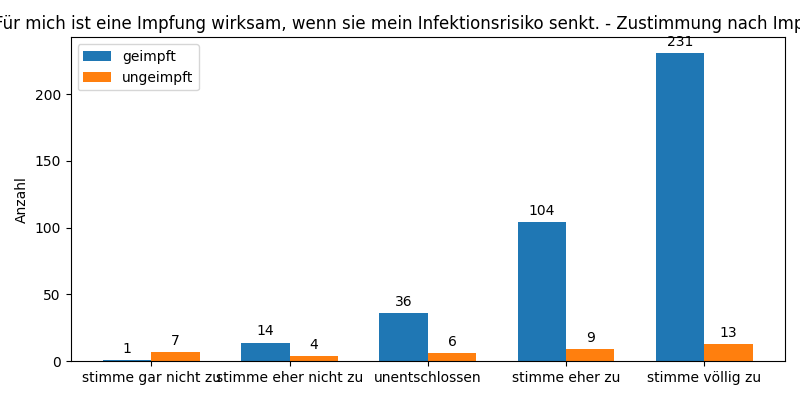
\includegraphics[trim={0 0 0 0.9cm},clip,width=.7\linewidth]{data_infektionsrisiko_impfstatus}
\end{figure}

\begin{figure}[ht]
    \caption{Für mich ist eine Impfung wirksam, wenn sie die Weitergabe des Krankheitserregers verhindert. - Nach Alter gruppiert}
    \label{fig:vgl_weitergabe_impfstatus}
    \centering
    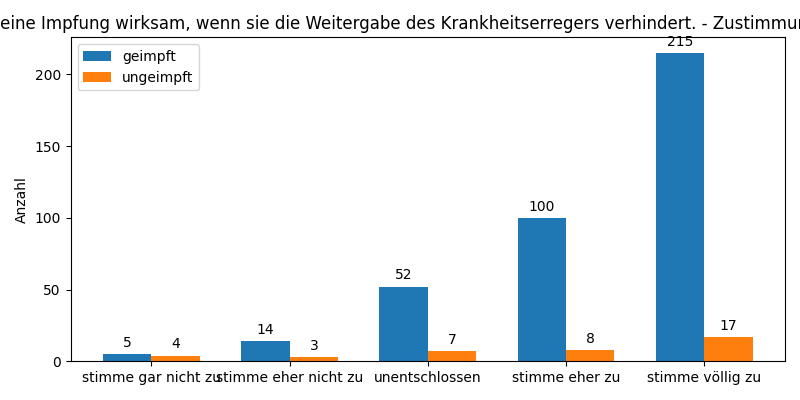
\includegraphics[trim={0 0 0 0.9cm},clip,width=.7\linewidth]{data_weitergabe_impfstatus}
\end{figure}

\begin{figure}[ht]
    \caption{Für mich ist eine Impfung wirksam, wenn sie im Falle einer Infektion meine Symptome mildert. - Nach Alter gruppiert}
    \label{fig:vgl_symptome_impfstatus}
    \centering
    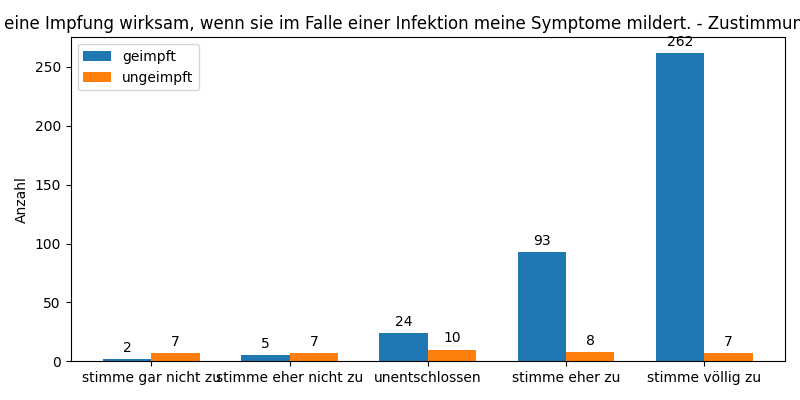
\includegraphics[trim={0 0 0 0.9cm},clip,width=.7\linewidth]{data_symptome_impfstatus}
\end{figure}

Weiters wurde die Nullhypothese angenommen, dass der Impfstatus einer Person keine Rolle spielt, ob man bereits Hygienemaßnahmen oder für ausreichend hält und ob man Maßnahmenverordnungen für wirksam hält.

Für erstere Nullhypothese wurde \(\chi^2 = 56,645\) mit einer Signifikanz von \(p = 0\), für zweitere \(\chi^2 = 105,903\) und \(p = 0\) errechnet. Damit werden beide Nullhypothesen abgelehnt, der hat also einen Einfluss auf genannte Ansichten.

Zuletzt wurde angenommen, dass der Impfstatus keinen Einfluss darauf hat, in welchen Bereichen man die COVID-19-Impfung für wirksam bzw. nicht wirksam hält. Die erste Hypothese wurde mit \(\chi^2 = 196,679\) und \(p = 0\) abgelehnt, die zweite Hypothese wurde mit \(\chi^2 = 7,815\) und \(p = 0,023\) ebenfalls abgelehnt. Der kritische Wert lag für diese Hypothesen bei 7,815.

\subsection{Zusammenhänge mit der Bildung}

Die Werte wurden in folgende Klassen eingeteilt:
\begin{itemize}
    \item Hochschule
    \item Matura
    \item Berufsbildende Mittlere Schule und Lehre
    \item Sonst
\end{itemize}

Als Nullhypothese \(H_0\) wird angenommen, dass die Bildungsstufe keinen Einfluss auf die Einschätzung der Wirksamkeit nimmt.

Der kritische Wert beträgt \(df = 21,026\) für eine Signifikanz \(p = 0,05\).
Für die erste Nullhypothese wurde \(\chi^2 = 19,770\) mit einer Signifikanz \(p = 0,072\) ermittelt. Für die zweite Nullhypothese wurde \(\chi^2 = 14,859\) mit einer Signifikanz \(p = 0,249\) berechnet. Für die dritte Nullhypothese ergibt \(\chi^2 = 19,421\) mit einer Signifikanz von \(p = 0,079\). Keine der drei Nullhypothesen kann abgelehnt werden, daraus folgt, dass die Bildung tatsächlich keine Auswirkung darauf hat, wie jemand die Wirksamkeit der Impfung einschätzt.

\begin{figure}[ht]
    \caption{Für mich ist eine Impfung wirksam, wenn sie mein Infektionsrisiko senkt. - Nach Bildung gruppiert}
    \label{fig:vgl_infektionsrisiko_bildung}
    \centering
    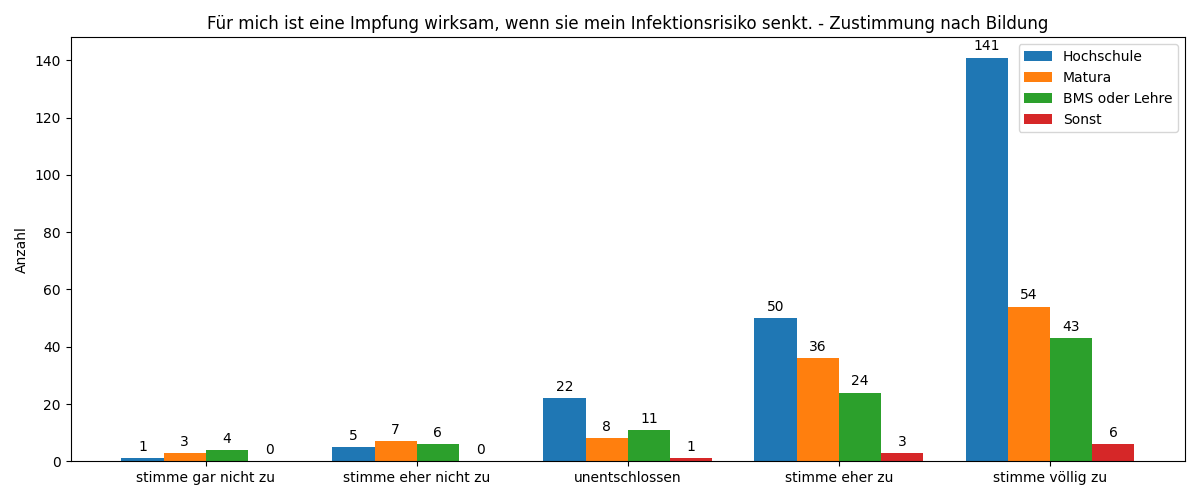
\includegraphics[trim={0 0 0 0.9cm},clip,width=.9\linewidth]{data_infektionsrisiko_bildung}
\end{figure}

\begin{figure}[ht]
    \caption{Für mich ist eine Impfung wirksam, wenn sie die Weitergabe des Krankheitserregers verhindert. - Nach Bildung gruppiert}
    \label{fig:vgl_weitergabe_bildung}
    \centering
    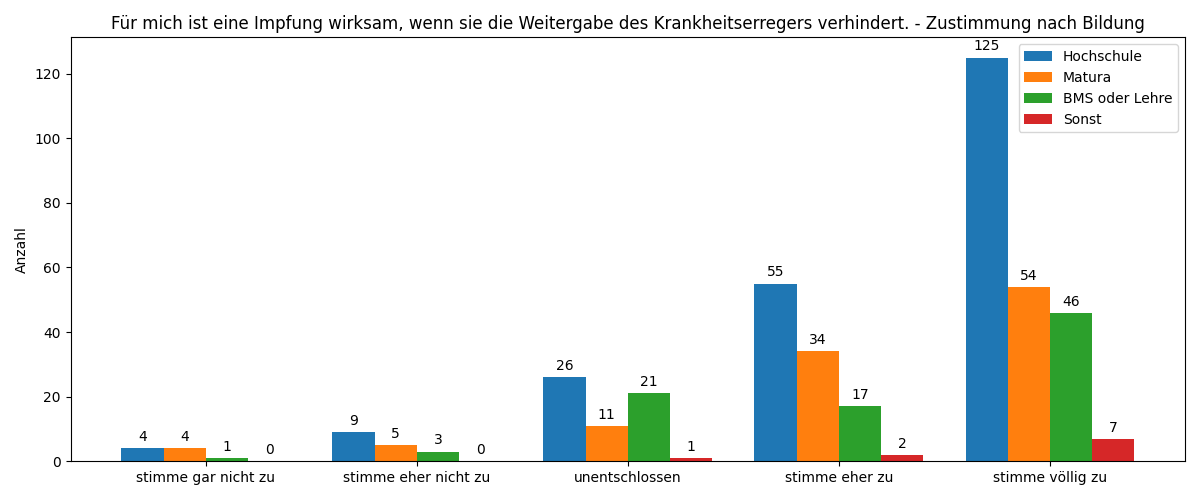
\includegraphics[trim={0 0 0 0.9cm},clip,width=.9\linewidth]{data_weitergabe_bildung}
\end{figure}

\begin{figure}[ht]
    \caption{Für mich ist eine Impfung wirksam, wenn sie im Falle einer Infektion meine Symptome mildert. - Nach Bildung gruppiert}
    \label{fig:vgl_symptome_bildung}
    \centering
    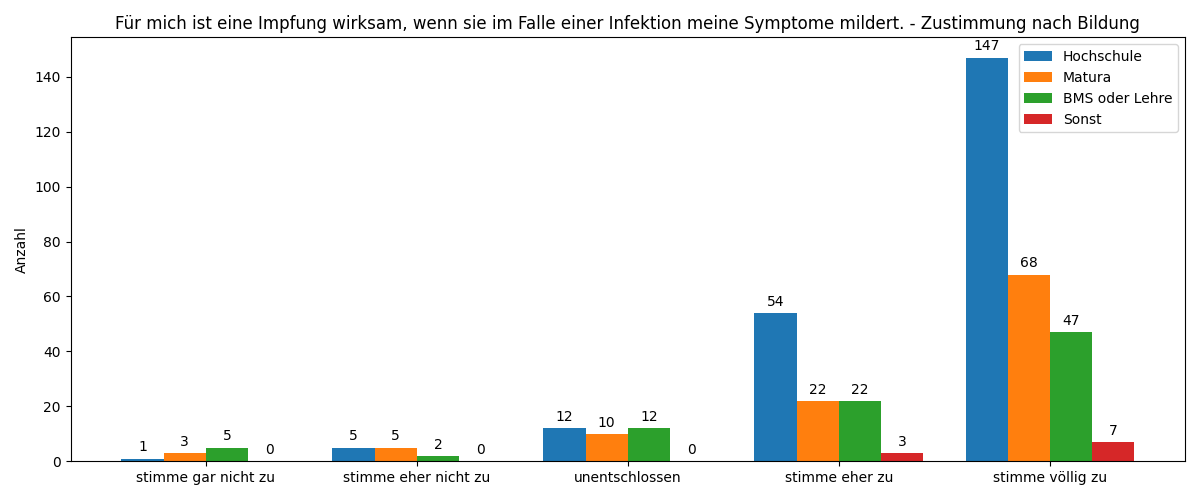
\includegraphics[trim={0 0 0 0.9cm},clip,width=.9\linewidth]{data_symptome_bildung}
\end{figure}

\subsection{Zusammenhänge mit dem Alter}

Die Werte wurden in folgende Altersklassen eingeteilt:
\begin{itemize}
    \item 0 bis 29 Jahre
    \item 30 bis 44 Jahre
    \item 45 bis 64 Jahre
    \item 65 Jahre oder älter
\end{itemize}
Als Nullhypothese \(H_0\) wird angenommen, dass das Alter keine Auswirkung auf die Einschätzung der Wirksamkeit hat.
Der kritische Wert beträgt \(df = 21,026\) für eine Signifikanz \(p = 0,05\). Bei der ersten Aussage ergab \(\chi^2 = 27,849\) mit einer Signifikanz \(p = 0,006\). Damit muss diese Nullhypothese abgelehnt werden.
Bei der zweiten Aussage konnte \(\chi^2 = 9,781\) mit einer Signifikanz von \(p = 0,635\) berechnet werden. Diese Nullhypothese kann folglich nicht abgelehnt werden.
Bei der dritten Aussage wurde  \(\chi^2 = 22,714\) mit einer Signifikanz von \(p = 0,03\) ermittelt. Diese Nullhypothese muss ebenfalls abgelehnt werden.

Damit wird die Nullhypothese abgelehnt, folglich gibt es einen Zusammenhang zwischen der Aussage "Für mich ist eine Impfung wirksam, wenn sie mein Infektionsrisiko senkt." und dem Alter.

Die zweite Nullhypothese -- das Alter hat keine Auswirkung auf die Zustimmung der Aussage "Für mich ist eine Impfung wirksam, wenn sie die Weitergabe des Krankheitserregers verhindert." -- wird beibehalten.

Die dritte Nullhypothese -- das Alter hat keine Auswirkung auf die Zustimmung der Aussage "Für mich ist eine Impfung wirksam, wenn sie im Falle einer Infektion meine Symptome mildert." -- wird abgelehnt.

\begin{figure}[ht]
    \caption{Für mich ist eine Impfung wirksam, wenn sie mein Infektionsrisiko senkt. - Nach Alter gruppiert}
    \label{fig:vgl_infektionsrisiko_altersgruppen}
    \centering
    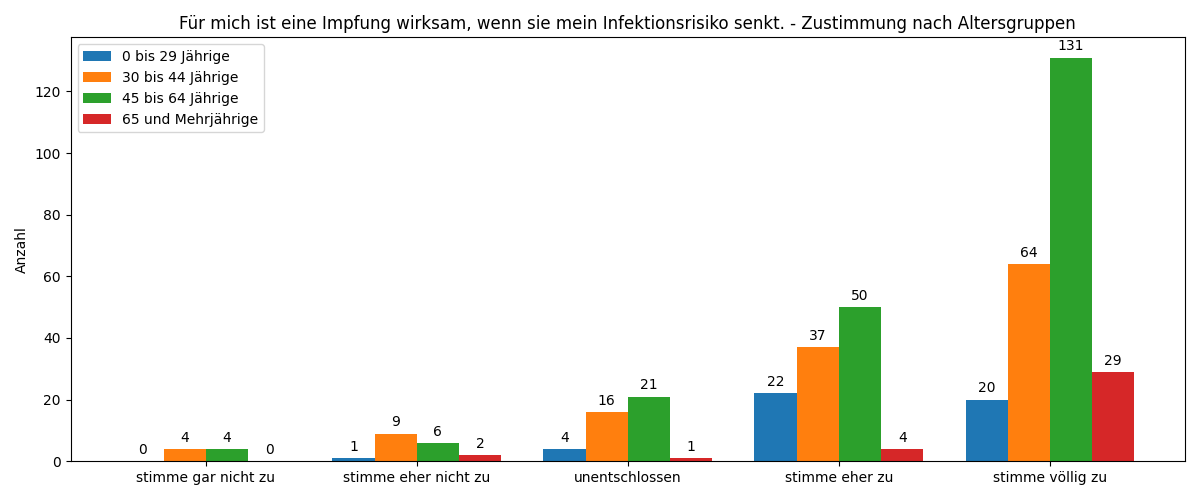
\includegraphics[trim={0 0 0 0.9cm},clip,width=.9\linewidth]{data_infektionsrisiko_altersgruppen}
\end{figure}

\begin{figure}[ht]
    \caption{Für mich ist eine Impfung wirksam, wenn sie die Weitergabe des Krankheitserregers verhindert. - Nach Alter gruppiert}
    \label{fig:vgl_weitergabe_altersgruppen}
    \centering
    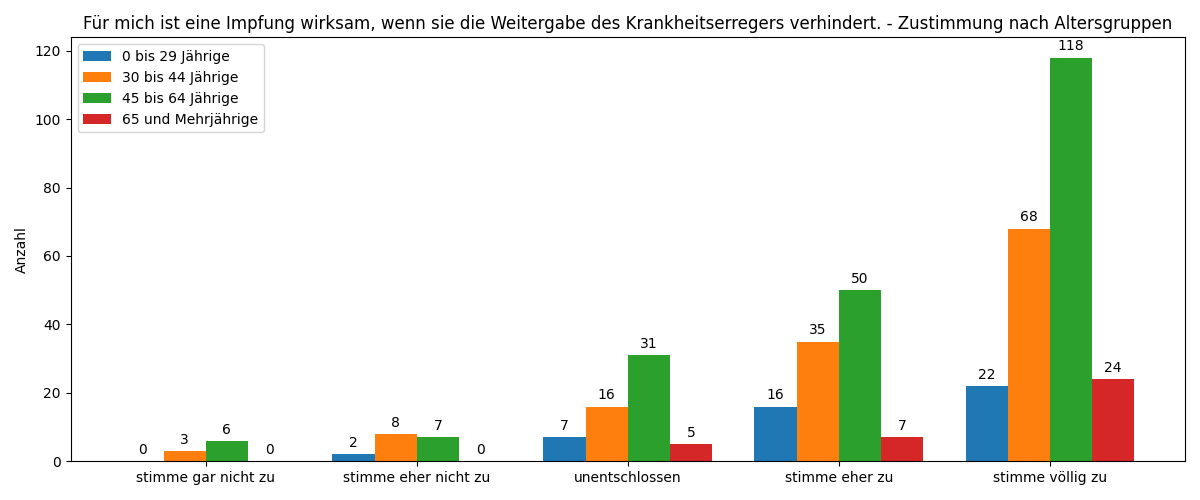
\includegraphics[trim={0 0 0 0.9cm},clip,width=.9\linewidth]{data_weitergabe_altersgruppen}
\end{figure}

\begin{figure}[ht]
    \caption{Für mich ist eine Impfung wirksam, wenn sie im Falle einer Infektion meine Symptome mildert. - Nach Alter gruppiert}
    \label{fig:vgl_symptome_altersgruppen}
    \centering
    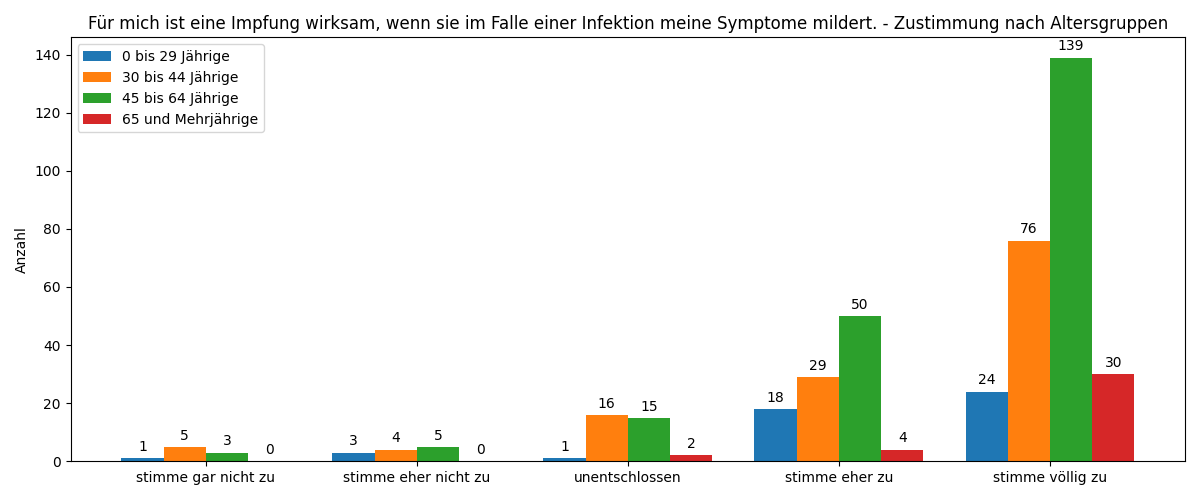
\includegraphics[trim={0 0 0 0.9cm},clip,width=.9\linewidth]{data_symptome_altersgruppen}
\end{figure}

\newpage

\section{Diskussion}

Es wurden Einflüsse des Alters und vor allem des Impfstatus auf die Einstellung bzw. Beurteilung der Maßnahmen und der Wirksamkeit der Impfung gezeigt. Die Bildung selber hatte dabei keinen entscheidenden Einfluss.
Interessant wäre dabei allerdings eine Beobachtung über längere Zeiträume und ob neue Erkenntnisse diese Meinung beeinflussen können.

\begin{table}[h!]
    \centering
    \begin{tabular} {p{9cm} | r | r | r}
        Nullhypothese & $\chi^2$ & p & Status \\
        \hline
        Der Impfstatus hat keinen Einfluss auf die Beurteilung der Wirksamkeit bzgl. Senkung des Infektionsrisikos. & 68,411 & 0,000 & abgelehnt \\
        Der Impfstatus hat keinen Einfluss auf die Beurteilung der Wirksamkeit bzgl. Weitergabe des Virus. & 16,764 & 0,002 & abgelehnt \\
        Der Impfstatus hat keinen Einfluss auf die Beurteilung der Wirksamkeit bzgl. Milderung der Symptome. & 116,457 & 0,000 & abgelehnt \\

        Der Impfstatus hat keinen Einfluss darauf, ob man einfache Hygienemaßnahmen als Maßnahme bereits für ausreichend hält. & 56,645 & 0,000 & abgelehnt \\
        Der Impfstatus hat keinen Einfluss darauf, ob man die Maßnahmenverordnung für wirksam hält. & 105,903 & 0,000 & abgelehnt \\

        Der Impfstatus hat keinen Einfluss darauf, in welchen Bereichen man die COVID-19-Impfung für wirksam hält. & 196,679 & 0,000 & abgelehnt \\
        Der Impfstatus hat keinen Einfluss darauf, in welchen Bereichen man die COVID-19-Impfung für nicht wirksam hält. & 9,552 & 0,023 & abgelehnt \\

        Die Bildung hat keinen Einfluss auf die Beurteilung der Wirksamkeit bzgl. Senkung des Infektionsrisikos. & 19,770 & 0,072 & angenommen \\
        Die Bildung hat keinen Einfluss auf die Beurteilung der Wirksamkeit bzgl. Weitergabe des Virus. & 14,859 & 0,249 & angenommen \\
        Die Bildung hat keinen Einfluss auf die Beurteilung der Wirksamkeit bzgl. Milderung der Symptome. & 19,421 & 0,000 & angenommen \\

        Das Alter hat keinen Einfluss auf die Beurteilung der Wirksamkeit bzgl. Senkung des Infektionsrisikos. & 27,849 & 0,006 & abgelehnt \\
        Das Alter hat keinen Einfluss auf die Beurteilung der Wirksamkeit bzgl. Weitergabe des Virus. & 9,781 & 0,635 & angenommen \\
        Das Alter hat keinen Einfluss auf die Beurteilung der Wirksamkeit bzgl. Milderung der Symptome. & 22,714 & 0,030 & abgelehnt \\

    \end{tabular}
    \caption{Aufgestellte Nullhypothesen - Übersicht}
    \label{tab:hypothesen}
\end{table}
% /* cSpell:disable */